\documentclass[]{article}
\usepackage{lmodern}
\usepackage{amssymb,amsmath}
\usepackage{ifxetex,ifluatex}
\usepackage{fixltx2e} % provides \textsubscript
\ifnum 0\ifxetex 1\fi\ifluatex 1\fi=0 % if pdftex
  \usepackage[T1]{fontenc}
  \usepackage[utf8]{inputenc}
\else % if luatex or xelatex
  \ifxetex
    \usepackage{mathspec}
  \else
    \usepackage{fontspec}
  \fi
  \defaultfontfeatures{Ligatures=TeX,Scale=MatchLowercase}
\fi
% use upquote if available, for straight quotes in verbatim environments
\IfFileExists{upquote.sty}{\usepackage{upquote}}{}
% use microtype if available
\IfFileExists{microtype.sty}{%
\usepackage{microtype}
\UseMicrotypeSet[protrusion]{basicmath} % disable protrusion for tt fonts
}{}
\usepackage[margin=1in]{geometry}
\usepackage{hyperref}
\hypersetup{unicode=true,
            pdftitle={Lab 01 Report},
            pdfauthor={YOUR NAME HERE},
            pdfborder={0 0 0},
            breaklinks=true}
\urlstyle{same}  % don't use monospace font for urls
\usepackage{color}
\usepackage{fancyvrb}
\newcommand{\VerbBar}{|}
\newcommand{\VERB}{\Verb[commandchars=\\\{\}]}
\DefineVerbatimEnvironment{Highlighting}{Verbatim}{commandchars=\\\{\}}
% Add ',fontsize=\small' for more characters per line
\usepackage{framed}
\definecolor{shadecolor}{RGB}{248,248,248}
\newenvironment{Shaded}{\begin{snugshade}}{\end{snugshade}}
\newcommand{\AlertTok}[1]{\textcolor[rgb]{0.94,0.16,0.16}{#1}}
\newcommand{\AnnotationTok}[1]{\textcolor[rgb]{0.56,0.35,0.01}{\textbf{\textit{#1}}}}
\newcommand{\AttributeTok}[1]{\textcolor[rgb]{0.77,0.63,0.00}{#1}}
\newcommand{\BaseNTok}[1]{\textcolor[rgb]{0.00,0.00,0.81}{#1}}
\newcommand{\BuiltInTok}[1]{#1}
\newcommand{\CharTok}[1]{\textcolor[rgb]{0.31,0.60,0.02}{#1}}
\newcommand{\CommentTok}[1]{\textcolor[rgb]{0.56,0.35,0.01}{\textit{#1}}}
\newcommand{\CommentVarTok}[1]{\textcolor[rgb]{0.56,0.35,0.01}{\textbf{\textit{#1}}}}
\newcommand{\ConstantTok}[1]{\textcolor[rgb]{0.00,0.00,0.00}{#1}}
\newcommand{\ControlFlowTok}[1]{\textcolor[rgb]{0.13,0.29,0.53}{\textbf{#1}}}
\newcommand{\DataTypeTok}[1]{\textcolor[rgb]{0.13,0.29,0.53}{#1}}
\newcommand{\DecValTok}[1]{\textcolor[rgb]{0.00,0.00,0.81}{#1}}
\newcommand{\DocumentationTok}[1]{\textcolor[rgb]{0.56,0.35,0.01}{\textbf{\textit{#1}}}}
\newcommand{\ErrorTok}[1]{\textcolor[rgb]{0.64,0.00,0.00}{\textbf{#1}}}
\newcommand{\ExtensionTok}[1]{#1}
\newcommand{\FloatTok}[1]{\textcolor[rgb]{0.00,0.00,0.81}{#1}}
\newcommand{\FunctionTok}[1]{\textcolor[rgb]{0.00,0.00,0.00}{#1}}
\newcommand{\ImportTok}[1]{#1}
\newcommand{\InformationTok}[1]{\textcolor[rgb]{0.56,0.35,0.01}{\textbf{\textit{#1}}}}
\newcommand{\KeywordTok}[1]{\textcolor[rgb]{0.13,0.29,0.53}{\textbf{#1}}}
\newcommand{\NormalTok}[1]{#1}
\newcommand{\OperatorTok}[1]{\textcolor[rgb]{0.81,0.36,0.00}{\textbf{#1}}}
\newcommand{\OtherTok}[1]{\textcolor[rgb]{0.56,0.35,0.01}{#1}}
\newcommand{\PreprocessorTok}[1]{\textcolor[rgb]{0.56,0.35,0.01}{\textit{#1}}}
\newcommand{\RegionMarkerTok}[1]{#1}
\newcommand{\SpecialCharTok}[1]{\textcolor[rgb]{0.00,0.00,0.00}{#1}}
\newcommand{\SpecialStringTok}[1]{\textcolor[rgb]{0.31,0.60,0.02}{#1}}
\newcommand{\StringTok}[1]{\textcolor[rgb]{0.31,0.60,0.02}{#1}}
\newcommand{\VariableTok}[1]{\textcolor[rgb]{0.00,0.00,0.00}{#1}}
\newcommand{\VerbatimStringTok}[1]{\textcolor[rgb]{0.31,0.60,0.02}{#1}}
\newcommand{\WarningTok}[1]{\textcolor[rgb]{0.56,0.35,0.01}{\textbf{\textit{#1}}}}
\usepackage{graphicx,grffile}
\makeatletter
\def\maxwidth{\ifdim\Gin@nat@width>\linewidth\linewidth\else\Gin@nat@width\fi}
\def\maxheight{\ifdim\Gin@nat@height>\textheight\textheight\else\Gin@nat@height\fi}
\makeatother
% Scale images if necessary, so that they will not overflow the page
% margins by default, and it is still possible to overwrite the defaults
% using explicit options in \includegraphics[width, height, ...]{}
\setkeys{Gin}{width=\maxwidth,height=\maxheight,keepaspectratio}
\IfFileExists{parskip.sty}{%
\usepackage{parskip}
}{% else
\setlength{\parindent}{0pt}
\setlength{\parskip}{6pt plus 2pt minus 1pt}
}
\setlength{\emergencystretch}{3em}  % prevent overfull lines
\providecommand{\tightlist}{%
  \setlength{\itemsep}{0pt}\setlength{\parskip}{0pt}}
\setcounter{secnumdepth}{0}
% Redefines (sub)paragraphs to behave more like sections
\ifx\paragraph\undefined\else
\let\oldparagraph\paragraph
\renewcommand{\paragraph}[1]{\oldparagraph{#1}\mbox{}}
\fi
\ifx\subparagraph\undefined\else
\let\oldsubparagraph\subparagraph
\renewcommand{\subparagraph}[1]{\oldsubparagraph{#1}\mbox{}}
\fi

%%% Use protect on footnotes to avoid problems with footnotes in titles
\let\rmarkdownfootnote\footnote%
\def\footnote{\protect\rmarkdownfootnote}

%%% Change title format to be more compact
\usepackage{titling}

% Create subtitle command for use in maketitle
\providecommand{\subtitle}[1]{
  \posttitle{
    \begin{center}\large#1\end{center}
    }
}

\setlength{\droptitle}{-2em}

  \title{Lab 01 Report}
    \pretitle{\vspace{\droptitle}\centering\huge}
  \posttitle{\par}
    \author{YOUR NAME HERE}
    \preauthor{\centering\large\emph}
  \postauthor{\par}
      \predate{\centering\large\emph}
  \postdate{\par}
    \date{DATE HERE}


\begin{document}
\maketitle

\hypertarget{skills}{%
\section{Skills}\label{skills}}

\begin{Shaded}
\begin{Highlighting}[]
\CommentTok{# load package of helpful datasets and functions}
\KeywordTok{library}\NormalTok{(tidyverse)}

\CommentTok{# load sleep dataset }
\KeywordTok{data}\NormalTok{(}\StringTok{"msleep"}\NormalTok{)}

\NormalTok{?msleep}

\CommentTok{# print out the first few rows}
\KeywordTok{head}\NormalTok{(msleep)}
\end{Highlighting}
\end{Shaded}

\begin{verbatim}
## # A tibble: 6 x 11
##   name  genus vore  order conservation sleep_total sleep_rem sleep_cycle
##   <chr> <chr> <chr> <chr> <chr>              <dbl>     <dbl>       <dbl>
## 1 Chee~ Acin~ carni Carn~ lc                  12.1      NA        NA    
## 2 Owl ~ Aotus omni  Prim~ <NA>                17         1.8      NA    
## 3 Moun~ Aplo~ herbi Rode~ nt                  14.4       2.4      NA    
## 4 Grea~ Blar~ omni  Sori~ lc                  14.9       2.3       0.133
## 5 Cow   Bos   herbi Arti~ domesticated         4         0.7       0.667
## 6 Thre~ Brad~ herbi Pilo~ <NA>                14.4       2.2       0.767
## # ... with 3 more variables: awake <dbl>, brainwt <dbl>, bodywt <dbl>
\end{verbatim}

Below is an example code chunk. Use chunks like these to run the Lab 01
code. You do not need to turn anything in for the Skills section of Lab
01.

\begin{Shaded}
\begin{Highlighting}[]
\CommentTok{# YOUR CODE HERE}
\end{Highlighting}
\end{Shaded}

\hypertarget{practice}{%
\section{Practice}\label{practice}}

\begin{enumerate}
\def\labelenumi{\arabic{enumi}.}
\tightlist
\item
  The \texttt{ChickWeight} dataset provides data on a sample of fifty
  chicks, each fed one of four different diets. For each chick, the data
  frame includes weight measurements at birth and every other day
  thereafter. Let's first take a look at the birth weights of the
  chicks. Here, we use the term in brackets
  \texttt{{[}ChickWeight\$Time\ ==\ 0{]}} to take a subset of our
  \texttt{ChickWeight\$weight} vector. The line below says we want all
  of the \texttt{weight} values in \texttt{ChickWeight} for which
  \texttt{Time\ ==\ 0}, meaning that the time is zero. We use the double
  equals sign \texttt{==} to test for equality.
\end{enumerate}

\begin{Shaded}
\begin{Highlighting}[]
\NormalTok{    ChickWeight}\OperatorTok{$}\NormalTok{weight[ChickWeight}\OperatorTok{$}\NormalTok{Time }\OperatorTok{==}\StringTok{ }\DecValTok{0}\NormalTok{]}
\end{Highlighting}
\end{Shaded}

\begin{verbatim}
##  [1] 42 40 43 42 41 41 41 42 42 41 43 41 41 41 41 41 42 39 43 41 40 41 43
## [24] 42 40 42 39 39 39 42 42 41 39 41 41 39 41 41 42 41 42 42 42 42 41 40
## [47] 41 39 40 41
\end{verbatim}

\begin{enumerate}
\def\labelenumi{\arabic{enumi}.}
\setcounter{enumi}{1}
\item
  The last day of the experiment is Day 21. Print out the ending weights
  of the chicks.
\item
  Calculate the mean ending weight of the chicks.
\item
  Next, let's take a look at the starting weights of the chicks that ate
  Diet 1. Below, the \texttt{\&} sign indicates that we want only the
  weight measurements that were from time zero \textbf{and} from chicks
  that ate Diet 1.
\end{enumerate}

\begin{Shaded}
\begin{Highlighting}[]
\NormalTok{    ChickWeight}\OperatorTok{$}\NormalTok{weight[ChickWeight}\OperatorTok{$}\NormalTok{Time }\OperatorTok{==}\StringTok{ }\DecValTok{0} \OperatorTok{&}\StringTok{ }\NormalTok{ChickWeight}\OperatorTok{$}\NormalTok{Diet }\OperatorTok{==}\StringTok{ }\DecValTok{1}\NormalTok{]}
\end{Highlighting}
\end{Shaded}

\begin{verbatim}
##  [1] 42 40 43 42 41 41 41 42 42 41 43 41 41 41 41 41 42 39 43 41
\end{verbatim}

\begin{enumerate}
\def\labelenumi{\arabic{enumi}.}
\setcounter{enumi}{4}
\item
  Print out the ending weights of the chicks that ate Diet 1.
\item
  For each diet, calculate the mean ending weight of the chicks that ate
  that diet. Is this a good way to compare the diets?
\item
  Make a histogram of all of the chicks' birthweights. Use the x-axis
  label ``Birth Weights'' and the title ``Frequency of Birthweights''.
  Provide a one-sentence summary of the plot.
\item
  Make a scatterplot with weight on the y-axis, and time on the x-axis.
  Use an appropriate title and axis labels, and change the color and
  shape of the points from their default values. Provide a one-sentence
  summary of the plot. Additionally, give one reason this is a good way
  to plot this data, and one reason this plot may be incomplete.
\item
  Finally, let's look at another way to subset our data. Below, we
  introduce the pipe operator \texttt{\%\textgreater{}\%}. The below
  code essentially says to take our \texttt{ChickWeight} data and
  include only the rows that satisfy \texttt{Diet\ ==\ 1}, and store it
  into a new data frame named \texttt{diet\_one}.
\end{enumerate}

\begin{Shaded}
\begin{Highlighting}[]
\NormalTok{    diet_one <-}\StringTok{ }\NormalTok{ChickWeight }\OperatorTok
\StringTok{      }\KeywordTok{filter}\NormalTok{(Diet }\OperatorTok{==}\StringTok{ }\DecValTok{1}\NormalTok{)}
\end{Highlighting}
\end{Shaded}

\begin{enumerate}
\def\labelenumi{\arabic{enumi}.}
\setcounter{enumi}{9}
\tightlist
\item
  The below line of code introduces a new plotting package called
  \texttt{ggplot2}, which can be difficult to learn at first but allows
  us to quickly produce complicated plots that display many variables at
  once. The first part \texttt{ggplot(diet\_one)} tells R we want to
  generate a ggplot based on the data in \texttt{diet\_one}. The
  \texttt{geom\_line()} function tells R we want to add line(s) to our
  plot. Finally, within \texttt{geom\_line()}, we provide aesthetics
  \texttt{aes(x\ =\ Time,\ y\ =\ weight,\ color\ =\ Chick)} that tell R
  we want the x-values for our lines to be times, the y-values to be
  weights, and the different colors should represent different chicks.
  \textbf{Provide a one-sentence summary of the resulting plot.}
\end{enumerate}

\begin{Shaded}
\begin{Highlighting}[]
    \KeywordTok{ggplot}\NormalTok{(diet_one) }\OperatorTok{+}\StringTok{ }\KeywordTok{geom_line}\NormalTok{(}\KeywordTok{aes}\NormalTok{(}\DataTypeTok{x =}\NormalTok{ Time, }\DataTypeTok{y =}\NormalTok{ weight, }\DataTypeTok{color =}\NormalTok{ Chick))}
\end{Highlighting}
\end{Shaded}

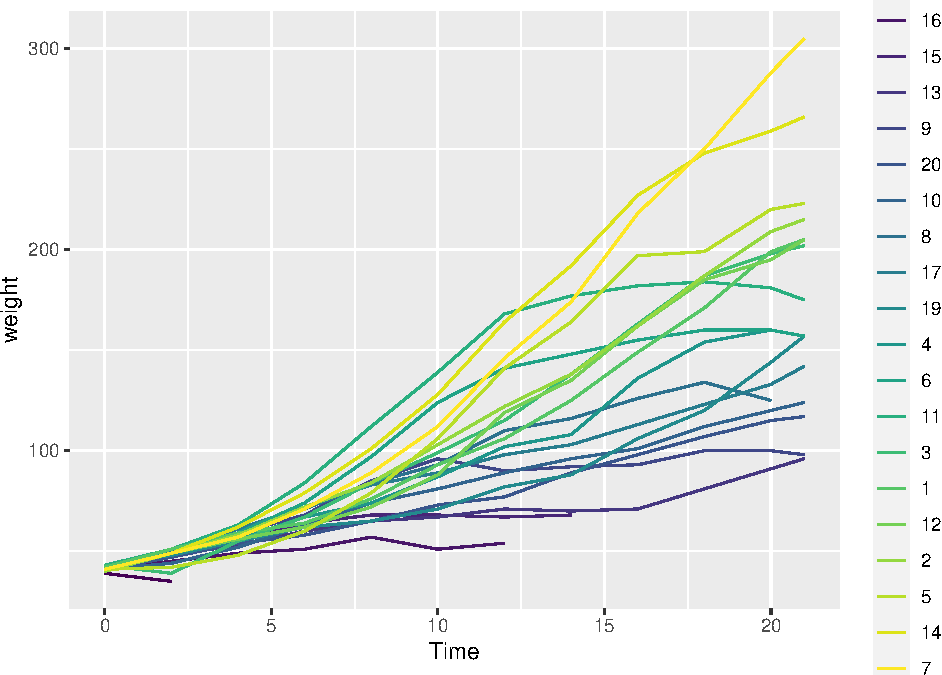
\includegraphics{lab_01_template_files/figure-latex/unnamed-chunk-11-1.pdf}

\begin{enumerate}
\def\labelenumi{\arabic{enumi}.}
\setcounter{enumi}{10}
\item
  Generate your own visualization of the \texttt{ChickWeight} data. You
  can use any of the functions we've used above, but you are encouraged
  to think about other kinds of plots and figure out how to make them in
  R. Provide a one-sentence summary of your plot. Additionally, give one
  reason this is a good way to plot this data, and one reason your plot
  may be incomplete.
\item
  Which diet produces the most weight gain? If you're not sure how to
  compute this in R, that is okay. If you can describe the set of steps
  you would take to compare the diets, that will be enough.
\end{enumerate}


\end{document}
